\documentclass[a4paper,11pt]{article}

%\usepackage{yfonts}
%\usepackage{unicode-math}
%\usepackage{fontspec}

\usepackage[round]{natbib}
\usepackage[english]{babel}
\selectlanguage{english}
\usepackage{numprint}

% Replace `letterpaper' with `a4paper' for UK/EU standard size
\usepackage[a4paper,top=2.5cm,bottom=2.5cm,left=3cm,right=3cm,marginparwidth=1.75cm]{geometry}

% Useful packages
\usepackage{graphicx} % Required for inserting images
\usepackage{latexsym,amsmath,amssymb,amscd,amsfonts,amsthm,mathrsfs,dsfont, txfonts}
\usepackage{tcolorbox}
\usepackage{xcolor}
\usepackage{amsbsy}
\usepackage{float}
\usepackage[colorlinks=true, allcolors=blue,breaklinks=true]{hyperref}
\usepackage[T1]{fontenc}
\usepackage{soul}
\usepackage{enumerate}
\usepackage{indentfirst}
\usepackage{booktabs}
\usepackage{multirow}
\usepackage{array}
\usepackage{appendix}
\usepackage{caption}
\usepackage{subcaption}
\usepackage{algorithm}
\usepackage{algpseudocode}

\graphicspath{ {./figures/} }

\newcommand{\rr}[1]{\textcolor{red}{#1}}
\newcommand{\ob}[1]{\colorbox{orange}{#1}}
\newcommand{\cb}[1]{\colorbox{cyan}{#1}}
\newcommand{\gb}[1]{\colorbox{lime}{#1}}
\newcommand{\yb}[1]{\colorbox{yellow}{#1}}

\newcommand{\nb}[1]{\yb{<begin NEW>}{#1}\yb{<end NEW>}}



\newcommand{\citeauth}[1]{\citeauthor{#1}, \citeyear{#1}}


\title{A data driven approach for optimal lineup building in Basket-Ball.}
\author{Arnaud ODET}
\date{Date TBD}


\begin{document}

\hbadness=99999  % suppresses underfull hbox warnings

\maketitle


\section*{Abstract}

\ob{To Do}

\section{Introduction}

\ob{To do}

\section{Related Work}

\ob{To do}

\section{Methodology}

\ob{To do}

\section{Results}
\label{sec:results}

\subsection{Clustering}

\subsubsection{Principal Component Analysis}

As specified in Section \ref{sec:data_trbs}, we performed a PCA to reduce the dimensionality of our dataset. 
We set an explained variance threshold target of 80\%, which corresponds to 14 principal components.
This thresholds returns a number of principal components 
Please refer to Table \ref{tab:pca} for further details about the principal components.

\begin{table}[htbp]
  \footnotesize
  \caption{Principal Component details}
  \label{tab:pca}
  \begin{tabular}{rrll}
\toprule
PC & EV* & Most Impacting Features & Description \\
\midrule
\multirow{2}{*}{1} & \multirow{2}{*}{0.240} & Drib. per touch ($\uparrow$), OREB contest\% ($\downarrow$), Pass. rec. ($\uparrow$), & Perimeter \\
& & Elbow touches ($\downarrow$), 2FG contest ($\downarrow$), Screen AST ($\downarrow$), FG3A ($\uparrow$) & ball handler \\
\midrule
\multirow{2}{*}{2} & \multirow{2}{*}{0.144} & Post FG\% ($\uparrow$), Min. ($\uparrow$), Elbow FG\% ($\uparrow$), Touches ($\uparrow$), Pass. rec. ($\uparrow$), & High usage \\
& & Pass. made ($\uparrow$), AST ($\uparrow$), Paint FG\% ($\uparrow$), USG\% ($\uparrow$) & inside player \\
\midrule
\multirow{2}{*}{3} & \multirow{2}{*}{0.088} & Elbow FG\% ($\uparrow$), Paint FG\% ($\uparrow$), Post FG\% ($\uparrow$), Min. ($\uparrow$), Pass. made ($\downarrow$), & Efficient shooter \\
& & Touches ($\downarrow$), Pass. rec. ($\downarrow$), FG3\% ($\uparrow$), Potential AST ($\downarrow$), FG3A ($\uparrow$) & with low poss. \\
\midrule
\multirow{2}{*}{4} & \multirow{2}{*}{0.058} & Post FG\% ($\uparrow$), Elbow FG\% ($\downarrow$), Paint FG\% ($\downarrow$), 2FG contest ($\downarrow$), & Poor defensive \\
& & Deflections ($\downarrow$), Def Boxouts ($\downarrow$), Post PTS ($\uparrow$), Screen AST ($\downarrow$), Min. ($\uparrow$) & post shoot \\ 
\midrule
5 & 0.045 & 2FG contest ($\uparrow$), Post FG\% ($\uparrow$), Def Boxouts ($\uparrow$), Deflections ($\uparrow$) & Inside defense \\ 
\midrule
6 & 0.040 & Post FG\% ($\uparrow$), Min. ($\downarrow$), Elbow FG\% ($\uparrow$), FG3A ($\downarrow$), FG3\% ($\downarrow$), Drive FG\% ($\downarrow$) & Inside shoot \\ 
\midrule
7 & 0.031 & Elbow FG\% ($\uparrow$), Paint FG\% ($\downarrow$), OREB contest\% ($\downarrow$), Drive FG\% ($\downarrow$) & Low hustle shoot \\ 
\midrule
8 & 0.029 & Drive FG\% ($\uparrow$), OREB contest\% ($\downarrow$), Pull-up FG\% ($\uparrow$), FG3A ($\downarrow$), FG2\% ($\uparrow$) & Shot creation \\ 
\midrule
9 & 0.027 & Paint FG\% ($\uparrow$), Elbow FG\% ($\downarrow$), Deflections ($\downarrow$), Catch \& shoot \% ($\uparrow$), FG3\% ($\uparrow$) & Catch \& shoot \\ 
\midrule
10 & 0.024 & OREB contest\% ($\uparrow$), Paint FG\% ($\downarrow$), Drive FG\% ($\uparrow$), Pass. made ($\uparrow$) & Outside shoot \& hustle \\ 
\midrule
11 & 0.023 & Min. ($\uparrow$), USG\% ($\downarrow$), Paint AST ($\uparrow$), FG3A ($\downarrow$), FG2A ($\downarrow$), Deflections ($\uparrow$) & High min., low resp. defense \\ 
\midrule
12 & 0.019 & Pull-up FG\% ($\uparrow$), Deflections ($\uparrow$), Def Rim FG\% ($\uparrow$), FG3A ($\downarrow$), STL ($\uparrow$) & Polyvalent defense \\ 
\midrule
13 & 0.018 & Def Rim FG\% ($\uparrow$), Deflections ($\downarrow$), Post AST ($\downarrow$), Drive FG\% ($\downarrow$), Min. ($\uparrow$) & Rim defense \\ 
\midrule
14 & 0.018 & Def Rim FG\% ($\uparrow$), Pull-up FG\% ($\downarrow$), Drive FG\% ($\uparrow$), Def Boxouts ($\uparrow$) & Inside defense \& shot creation \\ 
\bottomrule
\end{tabular}

  {\raggedright \small $\uparrow$ (respectively $\downarrow$) indicates feature positively (resp. negatively) correlated with the corresponding PC.}
\end{table}


\subsubsection{Clustering algorithms}

The Calinski-Harabasz indices of the compared method are presented in Figure \ref{fig:cl_ch}.
Please note that the number of clusters if for some algorithms (e.g. K-Means, GMM) an input hyperparameter, but for some others (e.g. Partition - HDBSCAN), it is a consequence of other hyperparameters.
\hl{A clear hierarchy emerges between algorithm : K-Means, GMM and Spherical K-Means consistently achieve top performance, while Agglomerative with Complete and Average linkage emerge as worst performers.
Agglomerative with Ward linkage and Partition HDBSCAN fall below the top three performers, the former appearing more constant (and better in most cluster sizes) than the latter.}
From this analysis, we will use K-Means as partition algorithm for the remaining of the paper.

\ob{Choose nb of clusters}

\begin{figure}[h]
  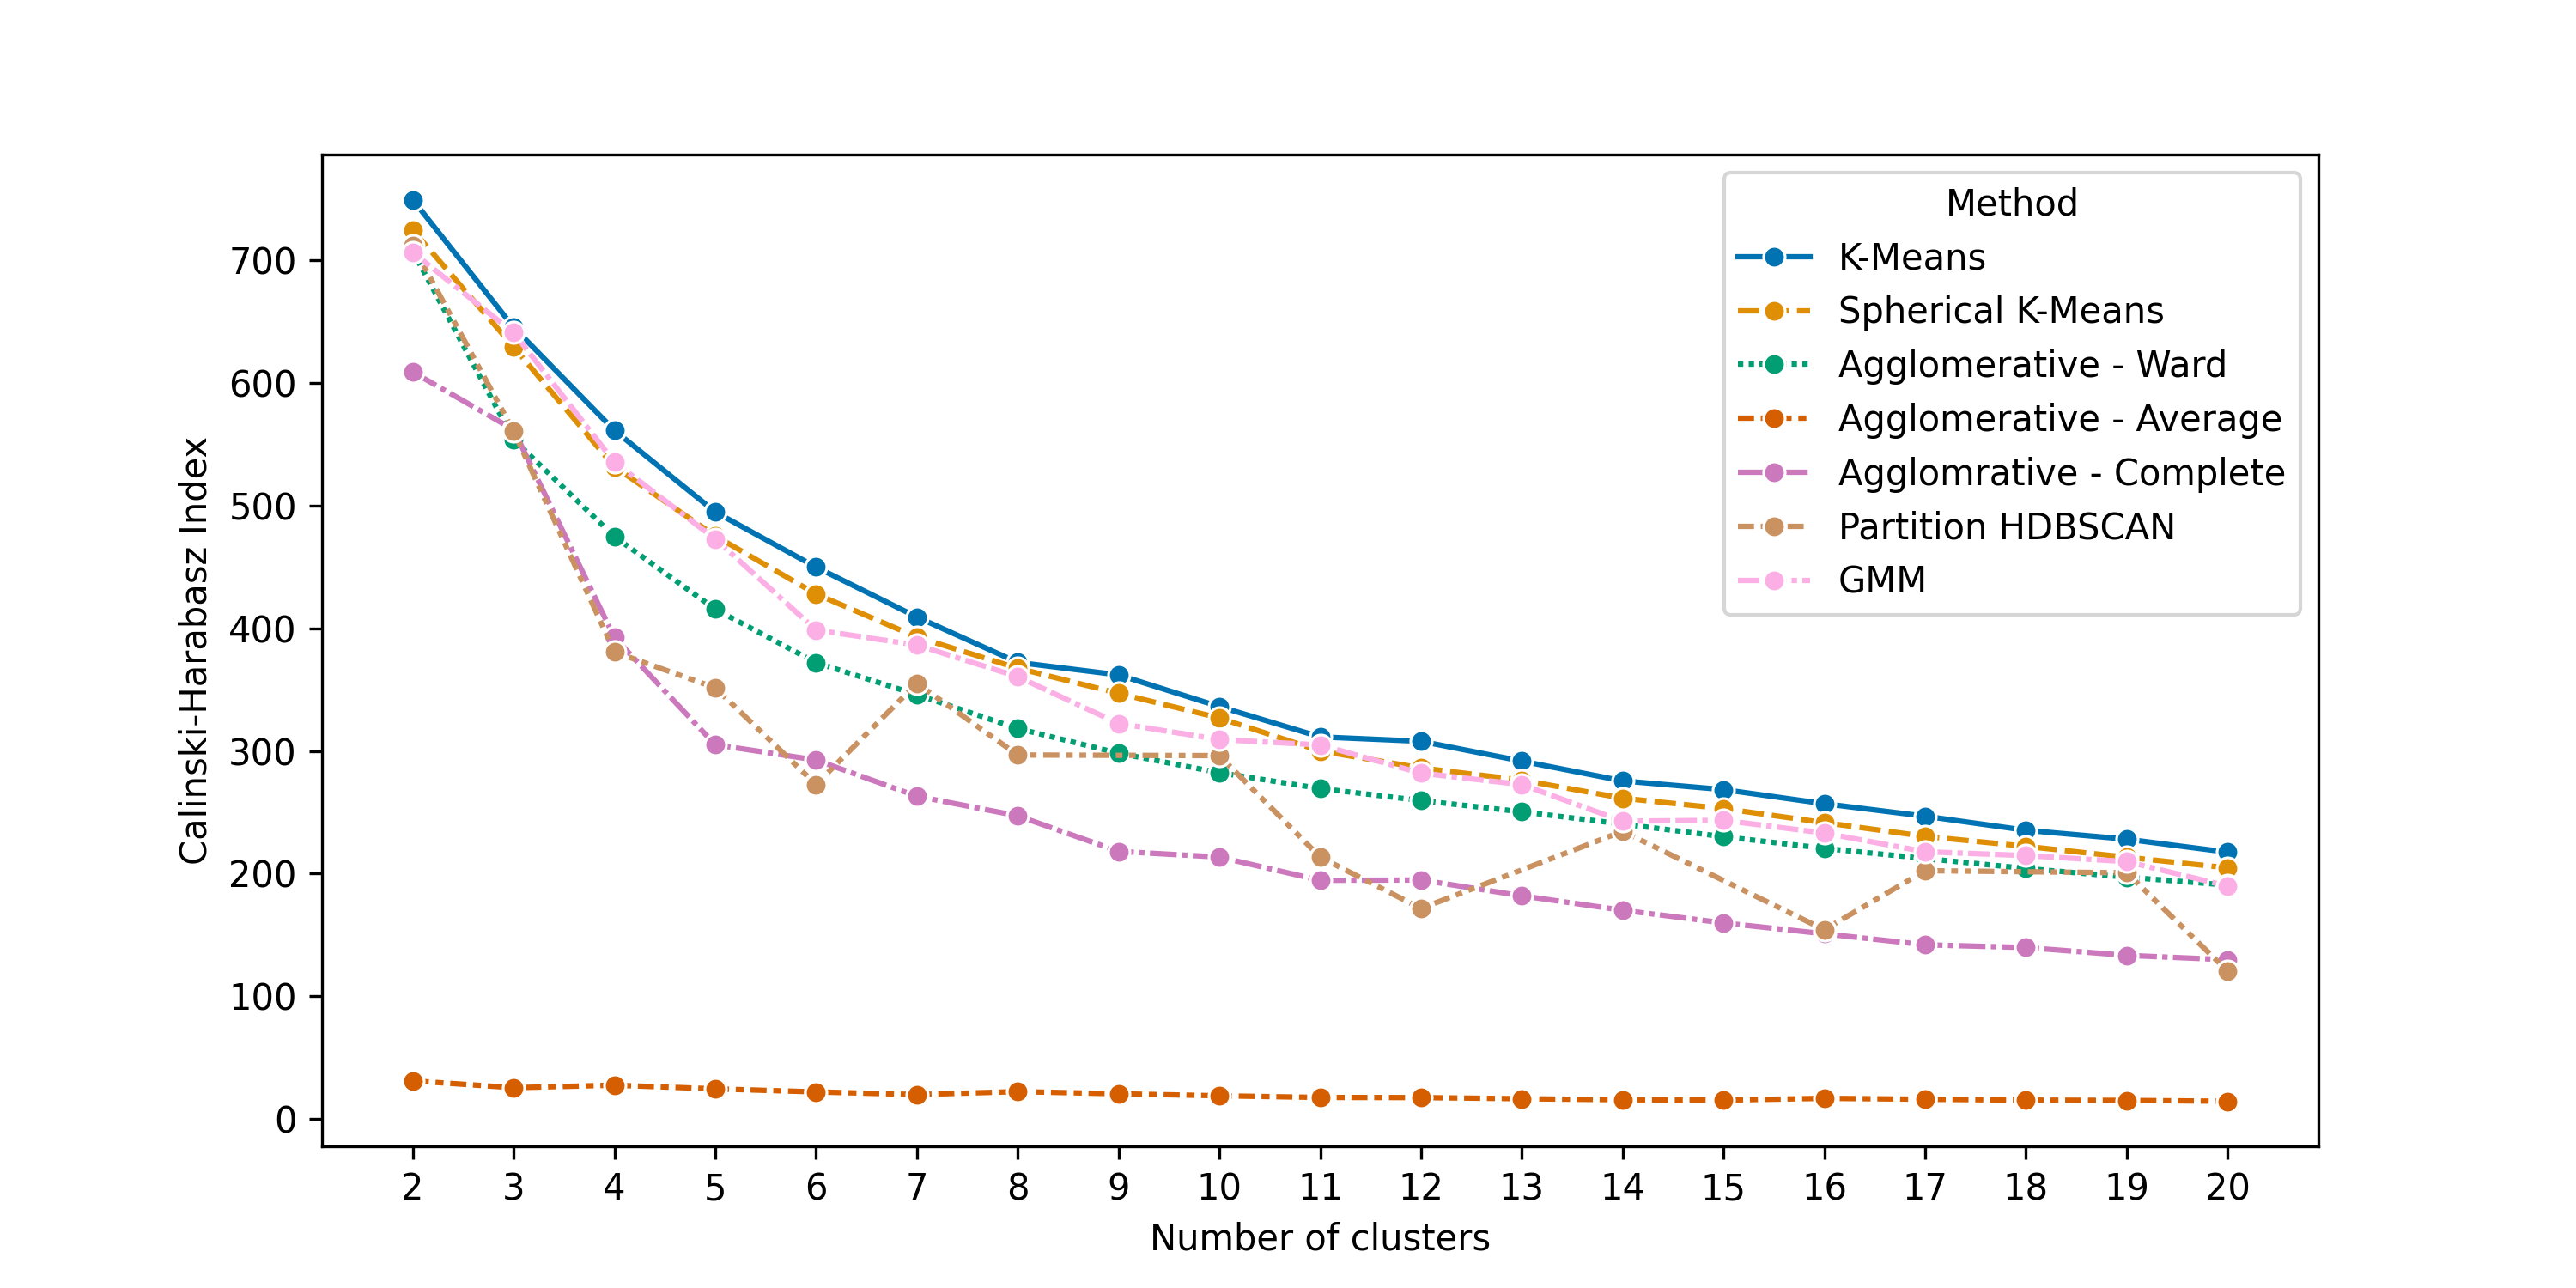
\includegraphics[width=\textwidth]{clustering_ch.png}  
  \caption{Comparison of clustering algorithm.}
  \label{fig:cl_ch}
\end{figure}

Figure \ref{fig:cl_viz} presents a visual inspection of the selected partition. 

\begin{figure}[h]
  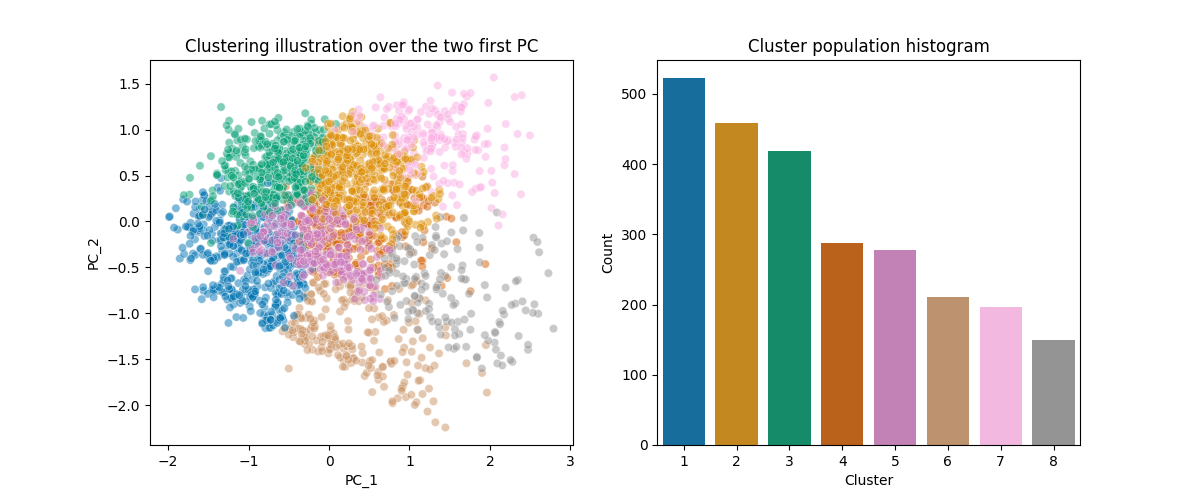
\includegraphics[width=\textwidth]{clustering_inspection.png}  
  \caption{Visualization of the selected partition. The left panel represents players in a 2D space determined by the two first principal components and the right panel a histogram of cluster populations.}
  \label{fig:cl_viz}
\end{figure}


\subsection{Roster Constitution}

\ob{To do}

\section{Discussion}
\label{sec:discuss}

\ob{To do}

Limitations : cluster stability, financial consideration, few seasons, bootstrapping issue (non explored space) 

Additivity vs symmetry

\ob{\cite{Fewell2012basketball}}

\section{Conclusion}

\ob{To do}


\bibliographystyle{apalike}
\bibliography{bibliography}

\pagebreak
\section*{Appendices}


\begin{table}[h!]
  \tiny
  \centering
  \caption{Comprehensive description of Principal Components in features space}
  \label{tab:app_pca}
  \begin{tabular}{lrrrrrrrrrrrrrr}
\toprule
Feature & PC 1 & PC 2 & PC 3 & PC 4 & PC 5 & PC 6 & PC 7 & PC 8 & PC 9 & PC 10 & PC 11 & PC 12 & PC 13 & PC 14 \\
\midrule
EFG PCT & -0.032 & 0.053 & 0.062 & -0.037 & 0.026 & -0.053 & -0.008 & 0.069 & 0.092 & -0.020 & -0.002 & -0.074 & 0.059 & -0.097 \\
USG PCT & 0.048 & 0.179 & -0.038 & 0.082 & -0.068 & -0.186 & -0.025 & -0.154 & -0.119 & -0.141 & -0.308 & -0.103 & 0.035 & -0.025 \\
MIN & 0.060 & 0.351 & 0.252 & 0.112 & -0.087 & -0.309 & -0.072 & -0.109 & -0.183 & -0.184 & 0.589 & -0.041 & 0.251 & 0.031 \\
PTS OFF TOV & 0.013 & 0.032 & 0.014 & 0.007 & -0.004 & -0.036 & -0.013 & -0.022 & -0.015 & -0.037 & -0.047 & -0.035 & 0.010 & -0.031 \\
PTS 2ND CHANCE & -0.112 & 0.058 & -0.025 & -0.011 & -0.045 & -0.050 & -0.031 & -0.056 & 0.010 & -0.080 & -0.113 & -0.080 & 0.096 & -0.120 \\
PTS FB & 0.023 & 0.021 & 0.024 & -0.003 & -0.012 & -0.012 & -0.042 & -0.016 & -0.034 & -0.029 & -0.034 & -0.027 & 0.018 & -0.035 \\
PTS PAINT & -0.094 & 0.144 & -0.080 & -0.040 & -0.065 & -0.019 & -0.155 & 0.010 & -0.100 & -0.151 & -0.171 & -0.114 & 0.060 & -0.096 \\
DRIVE PTS & 0.122 & 0.126 & -0.021 & -0.005 & 0.004 & -0.047 & -0.160 & 0.011 & -0.155 & -0.037 & -0.144 & -0.091 & 0.012 & -0.022 \\
DRIVE FG PCT & 0.019 & 0.175 & 0.082 & -0.043 & 0.014 & -0.236 & -0.275 & 0.700 & -0.151 & 0.252 & -0.063 & -0.215 & -0.255 & 0.244 \\
CATCH SHOOT PTS & 0.034 & -0.018 & 0.144 & 0.057 & 0.053 & -0.191 & 0.177 & -0.080 & 0.120 & 0.073 & -0.053 & -0.111 & -0.074 & -0.006 \\
CATCH SHOOT FG PCT & 0.017 & 0.088 & 0.141 & 0.014 & 0.013 & -0.168 & 0.160 & -0.012 & 0.215 & 0.113 & 0.047 & -0.229 & 0.092 & -0.188 \\
PULL UP PTS & 0.129 & 0.096 & 0.021 & 0.042 & 0.013 & -0.101 & -0.023 & -0.024 & -0.028 & -0.075 & -0.148 & 0.071 & 0.111 & -0.073 \\
PULL UP FG PCT & 0.073 & 0.117 & 0.129 & 0.049 & -0.007 & -0.222 & 0.052 & 0.291 & 0.131 & 0.101 & -0.191 & 0.668 & 0.186 & -0.415 \\
PAINT TOUCH PTS & -0.213 & 0.067 & -0.093 & -0.046 & -0.059 & 0.013 & -0.074 & 0.006 & 0.038 & -0.137 & -0.075 & -0.075 & 0.100 & -0.098 \\
PAINT TOUCH FG PCT & -0.095 & 0.182 & 0.262 & -0.304 & -0.037 & 0.050 & -0.397 & -0.136 & 0.626 & -0.291 & -0.055 & 0.066 & -0.168 & 0.176 \\
POST TOUCH PTS & -0.110 & 0.107 & -0.048 & 0.126 & -0.107 & -0.135 & 0.110 & -0.064 & -0.031 & -0.128 & -0.134 & 0.091 & -0.147 & 0.069 \\
POST TOUCH FG PCT & -0.217 & 0.363 & 0.261 & 0.621 & 0.378 & 0.457 & -0.009 & 0.041 & 0.019 & 0.009 & -0.076 & 0.011 & -0.043 & 0.029 \\
ELBOW TOUCH PTS & -0.097 & 0.059 & -0.021 & -0.042 & -0.058 & -0.005 & 0.077 & 0.034 & -0.025 & -0.029 & -0.065 & -0.040 & 0.047 & -0.045 \\
ELBOW TOUCH FG PCT & -0.049 & 0.297 & 0.450 & -0.539 & -0.104 & 0.305 & 0.422 & -0.013 & -0.317 & 0.046 & -0.115 & -0.002 & -0.048 & -0.005 \\
FG2A & -0.034 & 0.133 & -0.081 & 0.027 & -0.093 & -0.056 & -0.077 & -0.042 & -0.106 & -0.123 & -0.189 & -0.033 & 0.062 & -0.068 \\
FG2 PCT & -0.083 & 0.091 & 0.066 & -0.108 & -0.017 & 0.017 & -0.151 & 0.187 & 0.099 & -0.073 & -0.037 & -0.039 & 0.039 & -0.097 \\
FG3A & 0.182 & -0.050 & 0.197 & 0.070 & 0.191 & -0.287 & 0.148 & -0.229 & 0.057 & 0.044 & -0.195 & -0.133 & -0.134 & 0.112 \\
FG3 PCT & 0.121 & 0.051 & 0.200 & 0.035 & 0.108 & -0.254 & 0.101 & -0.045 & 0.208 & 0.178 & -0.010 & -0.141 & -0.058 & -0.152 \\
OFF LOSSES RECOV. & -0.012 & 0.028 & -0.024 & -0.089 & 0.174 & -0.072 & -0.077 & -0.028 & -0.106 & 0.008 & -0.069 & 0.020 & 0.054 & 0.145 \\
DEF LOSSES RECOV. & 0.009 & 0.002 & -0.010 & -0.037 & 0.078 & -0.024 & -0.013 & -0.020 & -0.046 & -0.015 & 0.001 & 0.029 & -0.008 & 0.057 \\
PFD & -0.022 & 0.119 & -0.063 & 0.018 & -0.043 & -0.067 & -0.064 & -0.042 & -0.101 & -0.087 & -0.088 & -0.047 & 0.062 & -0.021 \\
DRIVE PF & 0.080 & 0.079 & -0.018 & 0.012 & -0.019 & -0.025 & -0.114 & -0.050 & -0.127 & -0.037 & -0.102 & -0.076 & 0.027 & -0.025 \\
AVG SPEED OFF & 0.059 & -0.031 & 0.004 & -0.080 & 0.068 & 0.088 & -0.055 & 0.027 & 0.075 & 0.104 & -0.049 & -0.060 & 0.028 & -0.116 \\
AVG SPEED DEF & 0.005 & -0.061 & 0.010 & -0.047 & 0.007 & 0.071 & -0.038 & 0.043 & 0.001 & 0.007 & -0.004 & 0.026 & 0.010 & -0.046 \\
STL & 0.026 & 0.014 & -0.026 & -0.030 & 0.014 & 0.039 & -0.059 & -0.037 & -0.073 & -0.033 & 0.092 & 0.124 & -0.118 & 0.003 \\
BLK & -0.109 & 0.024 & -0.039 & -0.018 & -0.009 & -0.009 & -0.019 & -0.010 & -0.004 & -0.001 & 0.002 & -0.044 & -0.054 & -0.128 \\
DEF RIM FGM & -0.069 & 0.006 & -0.039 & -0.018 & 0.027 & -0.016 & 0.020 & -0.001 & 0.003 & 0.035 & -0.062 & 0.030 & 0.073 & 0.081 \\
DEF RIM FGA & -0.088 & 0.009 & -0.046 & -0.015 & 0.020 & -0.019 & 0.021 & 0.007 & 0.006 & 0.025 & -0.041 & -0.002 & 0.020 & 0.015 \\
DEF RIM FG PCT & 0.086 & 0.027 & 0.051 & -0.044 & 0.038 & -0.009 & -0.021 & -0.031 & 0.039 & 0.110 & -0.132 & 0.274 & 0.445 & 0.542 \\
D FGM & -0.050 & -0.031 & -0.073 & -0.019 & 0.033 & 0.022 & 0.019 & -0.020 & 0.009 & 0.013 & -0.118 & 0.016 & 0.015 & 0.056 \\
D FGA & -0.052 & -0.035 & -0.071 & -0.019 & 0.032 & 0.023 & 0.014 & -0.014 & 0.003 & 0.002 & -0.100 & 0.007 & -0.047 & -0.019 \\
D FG PCT & -0.008 & -0.002 & -0.020 & -0.002 & 0.010 & 0.001 & 0.022 & -0.016 & 0.007 & 0.027 & -0.053 & 0.037 & 0.126 & 0.161 \\
OPP PTS FB & -0.003 & 0.007 & -0.003 & 0.001 & -0.017 & 0.008 & 0.013 & 0.002 & -0.010 & -0.006 & -0.033 & -0.006 & 0.040 & 0.027 \\
OPP PTS PAINT & 0.006 & 0.004 & -0.001 & -0.018 & 0.051 & -0.027 & -0.009 & -0.018 & -0.031 & 0.002 & -0.061 & 0.030 & 0.107 & 0.107 \\
DEFLECTIONS & 0.022 & 0.029 & -0.036 & -0.144 & 0.279 & -0.051 & -0.145 & -0.085 & -0.219 & -0.082 & 0.187 & 0.341 & -0.325 & -0.036 \\
CHARGES DRAWN & 0.007 & 0.026 & -0.001 & -0.014 & 0.068 & -0.056 & 0.006 & -0.025 & -0.037 & -0.001 & 0.072 & 0.034 & -0.021 & 0.016 \\
CONTESTED SHOTS 2PT & -0.210 & 0.032 & -0.113 & -0.172 & 0.404 & -0.143 & 0.016 & -0.044 & -0.061 & -0.058 & -0.009 & 0.001 & -0.096 & -0.155 \\
CONTESTED SHOTS 3PT & -0.006 & -0.023 & 0.001 & -0.075 & 0.229 & -0.073 & -0.055 & -0.063 & -0.116 & -0.046 & -0.010 & 0.116 & -0.164 & -0.054 \\
SCREEN ASSISTS & -0.182 & 0.047 & -0.119 & -0.109 & 0.220 & -0.061 & 0.063 & 0.036 & 0.028 & -0.060 & 0.075 & -0.041 & 0.129 & -0.061 \\
SCREEN AST PTS & -0.201 & 0.051 & -0.131 & -0.121 & 0.248 & -0.066 & 0.069 & 0.038 & 0.030 & -0.066 & 0.087 & -0.049 & 0.140 & -0.067 \\
PAINT TOUCH PASSES & -0.114 & 0.025 & -0.073 & -0.019 & -0.059 & 0.052 & 0.003 & 0.045 & 0.029 & 0.030 & 0.073 & 0.006 & 0.030 & -0.043 \\
PAINT TOUCH AST & -0.080 & 0.093 & -0.040 & 0.007 & -0.043 & -0.047 & 0.000 & 0.039 & 0.004 & -0.028 & 0.224 & 0.028 & 0.034 & 0.017 \\
PAINT TOUCHES & -0.129 & 0.031 & -0.073 & -0.015 & -0.048 & 0.022 & -0.024 & 0.012 & -0.003 & -0.038 & -0.013 & -0.031 & 0.056 & -0.058 \\
POST TOUCH PASSES & -0.083 & 0.076 & -0.061 & 0.062 & -0.096 & -0.102 & 0.115 & -0.026 & -0.008 & -0.052 & -0.029 & 0.106 & -0.162 & 0.104 \\
POST TOUCH AST & -0.100 & 0.117 & -0.081 & 0.081 & -0.139 & -0.154 & 0.156 & -0.033 & 0.015 & -0.063 & 0.000 & 0.169 & -0.288 & 0.201 \\
POST TOUCHES & -0.120 & 0.105 & -0.076 & 0.107 & -0.143 & -0.151 & 0.146 & -0.062 & -0.030 & -0.106 & -0.104 & 0.126 & -0.197 & 0.103 \\
ELBOW TOUCH PASSES & -0.160 & 0.067 & -0.110 & 0.006 & -0.125 & -0.012 & 0.133 & 0.116 & 0.101 & 0.030 & 0.096 & 0.033 & 0.034 & 0.078 \\
ELBOW TOUCH AST & -0.088 & 0.055 & -0.071 & -0.008 & -0.056 & -0.037 & 0.099 & 0.056 & 0.077 & 0.006 & 0.072 & 0.029 & 0.021 & 0.073 \\
ELBOW TOUCHES & -0.225 & 0.101 & -0.135 & -0.003 & -0.157 & -0.029 & 0.151 & 0.125 & 0.065 & 0.007 & 0.031 & 0.006 & 0.072 & 0.039 \\
AST & 0.173 & 0.210 & -0.169 & -0.045 & 0.052 & 0.037 & 0.031 & -0.019 & 0.070 & 0.038 & 0.111 & 0.008 & -0.062 & 0.061 \\
FT AST & 0.023 & 0.022 & -0.021 & 0.005 & -0.016 & 0.020 & 0.005 & -0.011 & 0.008 & -0.004 & 0.013 & -0.007 & -0.011 & -0.011 \\
SECONDARY AST & 0.067 & 0.059 & -0.018 & -0.016 & 0.009 & 0.006 & 0.002 & -0.020 & 0.015 & 0.007 & 0.025 & -0.003 & 0.005 & -0.010 \\
POTENTIAL AST & 0.200 & 0.223 & -0.198 & -0.039 & 0.013 & 0.093 & 0.027 & -0.029 & 0.079 & 0.030 & 0.121 & 0.019 & -0.084 & 0.019 \\
PASSES MADE & 0.085 & 0.212 & -0.240 & -0.070 & 0.052 & 0.096 & 0.143 & 0.011 & 0.202 & 0.228 & 0.103 & -0.004 & -0.056 & 0.002 \\
PASSES RECEIVED & 0.226 & 0.248 & -0.209 & -0.029 & 0.020 & 0.039 & 0.078 & -0.038 & 0.099 & 0.058 & -0.046 & -0.024 & -0.018 & -0.016 \\
DRIVE PASSES & 0.113 & 0.071 & -0.052 & -0.032 & 0.023 & 0.035 & -0.052 & -0.023 & -0.023 & -0.008 & -0.023 & -0.027 & 0.013 & -0.014 \\
DRIVE AST & 0.062 & 0.042 & -0.031 & -0.014 & 0.011 & 0.016 & -0.023 & -0.008 & -0.002 & 0.009 & 0.001 & -0.030 & -0.002 & -0.014 \\
TOUCHES & 0.101 & 0.254 & -0.233 & -0.036 & 0.026 & 0.021 & 0.107 & -0.051 & 0.128 & 0.148 & -0.032 & -0.047 & -0.042 & -0.013 \\
AVG DRIB PER TOUCH & 0.350 & 0.178 & -0.180 & -0.051 & 0.043 & 0.144 & -0.117 & -0.004 & -0.057 & -0.061 & -0.075 & 0.000 & 0.092 & -0.096 \\
TOV & 0.026 & 0.091 & -0.102 & -0.000 & -0.017 & 0.001 & -0.014 & -0.054 & -0.048 & -0.030 & -0.095 & -0.042 & -0.018 & 0.031 \\
OREB UNCONTEST & -0.044 & 0.003 & -0.036 & -0.017 & 0.002 & 0.024 & 0.001 & 0.045 & 0.015 & -0.069 & 0.005 & -0.035 & 0.036 & -0.047 \\
OREB CONTEST PCT & -0.284 & 0.127 & 0.022 & -0.030 & -0.173 & -0.043 & -0.375 & -0.416 & -0.107 & 0.675 & 0.001 & 0.087 & -0.005 & -0.083 \\
OREB CHANCE DEFER & -0.021 & 0.061 & 0.005 & 0.007 & -0.027 & -0.024 & -0.028 & -0.017 & -0.048 & -0.020 & 0.102 & -0.017 & 0.079 & -0.047 \\
DREB CONTEST & -0.100 & 0.027 & -0.048 & 0.002 & -0.034 & -0.024 & 0.034 & -0.015 & 0.018 & 0.023 & -0.027 & -0.043 & -0.032 & -0.009 \\
DREB UNCONTEST & -0.076 & 0.052 & -0.048 & 0.001 & 0.001 & -0.042 & -0.007 & -0.043 & -0.019 & 0.014 & -0.010 & -0.047 & 0.034 & 0.035 \\
DREB CONTEST PCT & -0.144 & 0.011 & -0.027 & 0.013 & -0.067 & -0.022 & 0.052 & -0.002 & 0.030 & 0.089 & -0.042 & -0.051 & -0.113 & -0.040 \\
DREB CHANCE DEFER & -0.019 & -0.001 & -0.011 & 0.002 & 0.004 & -0.003 & 0.015 & -0.006 & 0.017 & 0.008 & 0.004 & -0.013 & 0.001 & -0.024 \\
OFF BOXOUTS & -0.073 & 0.019 & -0.043 & -0.034 & 0.090 & -0.039 & 0.011 & -0.008 & -0.015 & 0.023 & -0.029 & -0.030 & 0.125 & 0.043 \\
DEF BOXOUTS & -0.158 & 0.010 & -0.075 & -0.126 & 0.366 & -0.155 & 0.075 & -0.008 & 0.011 & 0.075 & -0.067 & -0.050 & 0.194 & 0.209 \\
\bottomrule
\end{tabular}

\end{table}


\begin{table}[h!]
  \centering
  \scriptsize
  \caption{Clusters' centroid position in Principal Component space}
  \label{tab:app_clust}
  \begin{tabular}{rrrrrrrrrrrrrrr}
\toprule
Cluster & PC 1 & PC 2 & PC 3 & PC 4 & PC 5 & PC 6 & PC 7 & PC 8 & PC 9 & PC 10 & PC 11 & PC 12 & PC 13 & PC 14 \\
\midrule
1 & -0.06 & 0.05 & 0.32 & 0.18 & 0.08 & 0.03 & -0.01 & -0.01 & -0.01 & 0.02 & 0.01 & 0.01 & -0.02 & 0.00 \\
2 & 0.16 & -0.28 & 0.28 & -0.25 & -0.07 & -0.06 & 0.03 & 0.01 & -0.02 & -0.01 & -0.00 & 0.01 & -0.01 & 0.02 \\
3 & 0.72 & 0.20 & -0.24 & -0.20 & -0.02 & 0.02 & -0.00 & 0.02 & 0.06 & 0.02 & 0.01 & 0.00 & 0.01 & -0.02 \\
4 & -0.78 & 0.17 & -0.14 & -0.10 & 0.16 & -0.03 & -0.02 & 0.13 & 0.00 & 0.03 & 0.02 & -0.03 & 0.06 & -0.03 \\
5 & 0.49 & 0.61 & 0.01 & 0.13 & 0.06 & 0.11 & -0.05 & -0.06 & -0.05 & -0.02 & 0.00 & -0.02 & 0.01 & -0.02 \\
6 & 0.08 & -0.51 & -0.10 & 0.05 & -0.00 & -0.12 & -0.21 & -0.08 & 0.13 & 0.04 & -0.01 & 0.02 & -0.03 & 0.03 \\
7 & 0.45 & -0.69 & -0.43 & 0.28 & 0.09 & -0.01 & 0.14 & 0.06 & -0.17 & -0.05 & -0.01 & -0.02 & -0.00 & -0.01 \\
8 & -0.48 & -0.00 & -0.05 & 0.16 & -0.50 & 0.16 & 0.03 & 0.09 & 0.08 & 0.08 & -0.02 & -0.01 & 0.01 & 0.00 \\
9 & -0.78 & -0.24 & -0.34 & -0.16 & 0.12 & 0.17 & 0.02 & -0.22 & 0.02 & -0.11 & -0.05 & -0.04 & 0.09 & -0.03 \\
10 & -0.59 & 0.61 & -0.21 & 0.14 & -0.18 & -0.31 & 0.17 & -0.07 & -0.02 & -0.09 & -0.01 & 0.09 & -0.15 & 0.10 \\
\bottomrule
\end{tabular}

\end{table}


\begin{table}[h!]
  \centering
  \tiny
  \caption{Clusters' centroid position in feature space}
  \label{tab:app_cl_ft}
  \begin{tabular}{lrrrrrrrrrr}
\toprule
cluster & 1 & 2 & 3 & 4 & 5 & 6 & 7 & 8 & 9 & 10 \\
\midrule
EFG PCT & 0.013 & 0.004 & -0.013 & 0.052 & 0.004 & -0.030 & -0.094 & -0.003 & -0.008 & 0.013 \\
USG PCT & -0.006 & -0.054 & 0.047 & -0.039 & 0.138 & -0.063 & -0.047 & -0.031 & -0.052 & 0.177 \\
MIN & 0.101 & -0.018 & 0.020 & -0.028 & 0.248 & -0.181 & -0.282 & -0.082 & -0.262 & 0.220 \\
PTS OFF TOV & 0.004 & -0.003 & 0.009 & -0.009 & 0.027 & -0.013 & -0.018 & -0.015 & -0.016 & 0.017 \\
PTS 2ND CHANCE & -0.010 & -0.036 & -0.060 & 0.096 & -0.019 & -0.029 & -0.087 & 0.060 & 0.111 & 0.100 \\
PTS FB & 0.005 & 0.006 & 0.014 & -0.019 & 0.029 & -0.008 & -0.015 & -0.016 & -0.024 & -0.012 \\
PTS PAINT & -0.030 & -0.065 & -0.017 & 0.110 & 0.049 & -0.066 & -0.117 & 0.054 & 0.092 & 0.132 \\
DRIVE PTS & -0.009 & -0.019 & 0.109 & -0.064 & 0.148 & -0.039 & -0.015 & -0.083 & -0.118 & -0.010 \\
DRIVE FG PCT & 0.024 & 0.003 & 0.032 & 0.103 & 0.057 & -0.067 & -0.135 & -0.005 & -0.322 & 0.074 \\
CATCH SHOOT PTS & 0.050 & 0.046 & -0.025 & -0.055 & -0.014 & 0.011 & -0.012 & -0.058 & -0.090 & 0.025 \\
CATCH SHOOT FG PCT & 0.041 & 0.016 & 0.008 & 0.004 & 0.036 & -0.050 & -0.120 & -0.016 & -0.092 & 0.026 \\
PULL UP PTS & 0.006 & -0.006 & 0.096 & -0.088 & 0.123 & -0.030 & 0.001 & -0.088 & -0.125 & 0.001 \\
PULL UP FG PCT & 0.039 & 0.013 & 0.056 & -0.015 & 0.058 & -0.053 & -0.092 & -0.026 & -0.230 & 0.050 \\
PAINT TOUCH PTS & -0.032 & -0.068 & -0.105 & 0.194 & -0.064 & -0.038 & -0.127 & 0.126 & 0.217 & 0.152 \\
PAINT TOUCH FG PCT & 0.039 & 0.063 & -0.010 & 0.057 & 0.028 & 0.029 & -0.528 & 0.014 & 0.042 & 0.063 \\
POST TOUCH PTS & 0.006 & -0.066 & -0.083 & 0.055 & 0.003 & -0.054 & -0.051 & 0.094 & 0.040 & 0.293 \\
POST TOUCH FG PCT & 0.273 & -0.269 & -0.276 & 0.177 & 0.269 & -0.249 & -0.258 & 0.083 & 0.007 & 0.177 \\
ELBOW TOUCH PTS & -0.014 & -0.021 & -0.044 & 0.090 & -0.024 & -0.064 & -0.071 & 0.072 & 0.075 & 0.102 \\
ELBOW TOUCH FG PCT & 0.065 & 0.180 & 0.012 & 0.042 & 0.108 & -0.387 & -0.475 & 0.003 & -0.059 & 0.045 \\
FG2A & -0.024 & -0.061 & 0.009 & 0.039 & 0.071 & -0.057 & -0.058 & 0.043 & 0.034 & 0.141 \\
FG2 PCT & 0.005 & -0.000 & -0.025 & 0.109 & -0.002 & -0.044 & -0.181 & 0.045 & 0.016 & 0.020 \\
FG3A & 0.069 & 0.089 & 0.044 & -0.188 & 0.050 & 0.060 & 0.069 & -0.233 & -0.186 & -0.057 \\
FG3 PCT & 0.066 & 0.053 & 0.052 & -0.090 & 0.064 & 0.006 & -0.072 & -0.129 & -0.208 & -0.035 \\
OFF LOSSES RECOV. & -0.009 & -0.001 & 0.007 & 0.053 & 0.011 & -0.002 & -0.021 & -0.117 & 0.037 & 0.006 \\
DEF LOSSES RECOV. & -0.004 & 0.005 & 0.011 & 0.006 & 0.006 & 0.002 & 0.008 & -0.061 & 0.008 & -0.003 \\
PFD & -0.017 & -0.051 & 0.012 & 0.037 & 0.068 & -0.051 & -0.052 & 0.010 & 0.018 & 0.116 \\
DRIVE PF & -0.006 & -0.016 & 0.067 & -0.053 & 0.102 & -0.022 & -0.003 & -0.048 & -0.063 & -0.005 \\
AVG SPEED OFF & -0.010 & 0.021 & 0.061 & -0.023 & 0.013 & 0.024 & 0.007 & -0.045 & -0.011 & -0.147 \\
AVG SPEED DEF & -0.006 & 0.025 & 0.002 & -0.004 & -0.033 & 0.024 & 0.023 & 0.001 & 0.018 & -0.085 \\
STL & -0.007 & -0.001 & 0.028 & -0.023 & 0.028 & 0.001 & 0.006 & -0.034 & -0.012 & 0.006 \\
BLK & -0.009 & -0.032 & -0.059 & 0.096 & -0.038 & -0.016 & -0.054 & 0.053 & 0.096 & 0.078 \\
DEF RIM FGM & -0.011 & -0.020 & -0.037 & 0.067 & -0.035 & -0.005 & -0.021 & 0.021 & 0.071 & 0.051 \\
DEF RIM FGA & -0.012 & -0.026 & -0.048 & 0.083 & -0.043 & -0.009 & -0.026 & 0.034 & 0.083 & 0.067 \\
DEF RIM FG PCT & 0.006 & 0.031 & 0.060 & -0.058 & 0.044 & 0.012 & -0.039 & -0.059 & -0.071 & -0.055 \\
D FGM & -0.023 & -0.018 & -0.023 & 0.045 & -0.044 & 0.017 & 0.028 & 0.015 & 0.090 & 0.020 \\
D FGA & -0.022 & -0.017 & -0.025 & 0.045 & -0.046 & 0.018 & 0.031 & 0.015 & 0.088 & 0.020 \\
D FG PCT & -0.007 & -0.005 & -0.003 & 0.010 & -0.008 & 0.003 & 0.004 & 0.004 & 0.023 & 0.008 \\
OPP PTS FB & -0.003 & -0.002 & -0.000 & 0.001 & 0.003 & -0.009 & -0.002 & 0.012 & 0.005 & 0.006 \\
OPP PTS PAINT & -0.002 & 0.003 & 0.004 & 0.007 & 0.005 & 0.001 & 0.001 & -0.038 & 0.010 & -0.007 \\
DEFLECTIONS & -0.005 & 0.011 & 0.037 & 0.021 & 0.037 & 0.006 & -0.003 & -0.228 & 0.008 & 0.025 \\
CHARGES DRAWN & 0.003 & -0.003 & 0.008 & 0.009 & 0.018 & -0.011 & -0.009 & -0.056 & -0.013 & 0.026 \\
CONTESTED SHOTS 2PT & -0.028 & -0.051 & -0.097 & 0.264 & -0.089 & -0.028 & -0.065 & -0.163 & 0.259 & 0.126 \\
CONTESTED SHOTS 3PT & 0.006 & 0.015 & -0.009 & 0.029 & -0.011 & 0.020 & 0.021 & -0.159 & 0.036 & -0.008 \\
SCREEN ASSISTS & -0.035 & -0.062 & -0.072 & 0.230 & -0.069 & -0.048 & -0.065 & -0.043 & 0.217 & 0.108 \\
SCREEN AST PTS & -0.039 & -0.068 & -0.080 & 0.254 & -0.077 & -0.053 & -0.070 & -0.050 & 0.240 & 0.116 \\
PAINT TOUCH PASSES & -0.022 & -0.042 & -0.049 & 0.105 & -0.045 & -0.023 & -0.051 & 0.101 & 0.101 & 0.075 \\
PAINT TOUCH AST & -0.006 & -0.045 & -0.028 & 0.087 & 0.009 & -0.050 & -0.084 & 0.052 & 0.026 & 0.131 \\
PAINT TOUCHES & -0.022 & -0.046 & -0.064 & 0.116 & -0.043 & -0.024 & -0.056 & 0.089 & 0.128 & 0.091 \\
POST TOUCH PASSES & -0.009 & -0.045 & -0.049 & 0.044 & -0.013 & -0.039 & -0.036 & 0.080 & 0.023 & 0.237 \\
POST TOUCH AST & -0.011 & -0.059 & -0.056 & 0.047 & -0.009 & -0.050 & -0.060 & 0.105 & 0.003 & 0.346 \\
POST TOUCHES & -0.008 & -0.065 & -0.080 & 0.058 & -0.014 & -0.054 & -0.047 & 0.115 & 0.043 & 0.330 \\
ELBOW TOUCH PASSES & -0.034 & -0.064 & -0.067 & 0.145 & -0.067 & -0.055 & -0.073 & 0.167 & 0.100 & 0.200 \\
ELBOW TOUCH AST & -0.023 & -0.039 & -0.029 & 0.086 & -0.032 & -0.037 & -0.051 & 0.080 & 0.054 & 0.138 \\
ELBOW TOUCHES & -0.043 & -0.085 & -0.101 & 0.204 & -0.081 & -0.086 & -0.108 & 0.210 & 0.155 & 0.268 \\
AST & -0.054 & -0.073 & 0.219 & -0.069 & 0.207 & -0.074 & -0.015 & -0.097 & -0.121 & 0.053 \\
FT AST & -0.007 & -0.010 & 0.026 & -0.017 & 0.027 & -0.009 & 0.003 & 0.001 & -0.013 & 0.003 \\
SECONDARY AST & -0.008 & -0.009 & 0.069 & -0.038 & 0.068 & -0.022 & -0.011 & -0.038 & -0.052 & -0.006 \\
POTENTIAL AST & -0.063 & -0.083 & 0.249 & -0.094 & 0.233 & -0.080 & -0.003 & -0.080 & -0.130 & 0.042 \\
PASSES MADE & -0.073 & -0.108 & 0.190 & 0.020 & 0.151 & -0.086 & -0.045 & -0.014 & -0.033 & 0.090 \\
PASSES RECEIVED & -0.070 & -0.089 & 0.274 & -0.105 & 0.255 & -0.091 & 0.005 & -0.094 & -0.145 & 0.052 \\
DRIVE PASSES & -0.022 & -0.014 & 0.113 & -0.063 & 0.105 & -0.020 & 0.012 & -0.068 & -0.067 & -0.043 \\
DRIVE AST & -0.012 & -0.010 & 0.064 & -0.033 & 0.059 & -0.011 & 0.006 & -0.034 & -0.041 & -0.021 \\
TOUCHES & -0.069 & -0.116 & 0.194 & -0.002 & 0.191 & -0.098 & -0.052 & -0.031 & -0.050 & 0.137 \\
AVG DRIB PER TOUCH & -0.072 & -0.047 & 0.343 & -0.203 & 0.302 & -0.054 & 0.096 & -0.176 & -0.200 & -0.154 \\
TOV & -0.031 & -0.047 & 0.056 & -0.004 & 0.073 & -0.033 & -0.003 & -0.007 & 0.008 & 0.072 \\
OREB UNCONTEST & -0.014 & -0.016 & -0.017 & 0.050 & -0.019 & -0.013 & -0.007 & 0.024 & 0.057 & 0.014 \\
OREB CONTEST PCT & 0.037 & -0.075 & -0.175 & 0.187 & -0.045 & 0.035 & -0.340 & 0.206 & 0.164 & 0.185 \\
OREB CHANCE DEFER & 0.005 & -0.018 & -0.006 & 0.028 & 0.031 & -0.035 & -0.051 & 0.011 & 0.001 & 0.041 \\
DREB CONTEST & -0.011 & -0.033 & -0.055 & 0.081 & -0.039 & -0.017 & -0.044 & 0.068 & 0.082 & 0.104 \\
DREB UNCONTEST & -0.009 & -0.039 & -0.036 & 0.074 & -0.006 & -0.021 & -0.049 & 0.029 & 0.067 & 0.095 \\
DREB CONTEST PCT & -0.001 & -0.031 & -0.096 & 0.102 & -0.075 & -0.013 & -0.061 & 0.115 & 0.094 & 0.128 \\
DREB CHANCE DEFER & -0.002 & -0.007 & -0.010 & 0.017 & -0.010 & -0.000 & -0.003 & 0.009 & 0.021 & 0.011 \\
OFF BOXOUTS & -0.011 & -0.026 & -0.034 & 0.091 & -0.025 & -0.015 & -0.026 & -0.018 & 0.087 & 0.038 \\
DEF BOXOUTS & -0.018 & -0.034 & -0.080 & 0.219 & -0.088 & -0.011 & -0.044 & -0.138 & 0.195 & 0.074 \\
\bottomrule
\end{tabular}

\end{table}


\begin{table}[!htb]
  \footnotesize
  \caption{Valid and statistically significant combinations of players}
  \label{tab:app_comb}
  \begin{minipage}[t]{.3\linewidth}
    \caption{3 players}
    \centering
    \label{tab:app_comb_3}
    \begin{tabular}{lrrr}
Lineup & $n_w$ & time & $\hat{S}_{lineup}$ \\
5-9-10 & 37 & 1,675 & 10.3 \\
1-9-10 & 34 & 1,356 & 9.8 \\
3-3-5 & 100 & 3,068 & 6.5 \\
3-5-5 & 192 & 8,788 & 5.6 \\
5-5-10 & 375 & 20,562 & 5.2 \\
2-5-5 & 700 & 32,570 & 4.1 \\
5-8-10 & 198 & 10,672 & 3.4 \\
1-5-10 & 1,565 & 78,312 & 3.3 \\
2-2-10 & 536 & 20,890 & 3.2 \\
1-5-5 & 1,117 & 62,022 & 3.2 \\
4-5-5 & 739 & 41,943 & 2.9 \\
3-3-4 & 411 & 15,339 & 2.7 \\
2-5-10 & 1,175 & 54,080 & 2.6 \\
2-5-8 & 526 & 24,047 & 2.5 \\
2-2-5 & 962 & 36,134 & 2.2 \\
4-5-10 & 546 & 29,798 & 2.2 \\
1-2-5 & 2,494 & 103,270 & 1.9 \\
1-2-10 & 1,338 & 56,499 & 1.5 \\
1-5-8 & 873 & 42,150 & 1.5 \\
1-1-10 & 1,194 & 56,106 & 1.3 \\
1-3-5 & 1,650 & 64,766 & 1.2 \\
2-3-4 & 1,640 & 53,337 & -1.5 \\
1-2-3 & 2,206 & 71,554 & -1.6 \\
1-1-8 & 779 & 32,071 & -1.8 \\
1-3-4 & 2,399 & 91,008 & -2.0 \\
1-1-1 & 1,082 & 48,573 & -2.0 \\
1-1-4 & 1,963 & 88,367 & -2.3 \\
3-8-10 & 210 & 8,701 & -2.9 \\
5-8-8 & 368 & 16,683 & -3.2 \\
1-1-3 & 2,365 & 88,356 & -3.3 \\
1-3-8 & 733 & 24,696 & -3.5 \\
2-3-8 & 385 & 10,723 & -3.6 \\
4-4-5 & 228 & 8,356 & -3.7 \\
3-4-4 & 305 & 9,354 & -3.7 \\
3-3-8 & 97 & 3,260 & -3.9 \\
1-1-9 & 245 & 7,629 & -3.9 \\
1-8-8 & 431 & 18,717 & -4.7 \\
3-8-8 & 315 & 11,129 & -4.8 \\
6-8-8 & 82 & 2,202 & -4.8 \\
1-4-4 & 334 & 10,498 & -5.5 \\
4-4-6 & 47 & 934 & -10.0 \\
\end{tabular}

  \end{minipage}%
  \hfill
  \begin{minipage}[t]{.01\linewidth}
  \end{minipage}%
  \hfill\vline\hfill
  \begin{minipage}[t]{.3\linewidth}
    \centering
      \caption{4 players}
      \label{tab:app_comb_4}
      \begin{tabular}{lrr}
  \toprule
  Lineup & $n_w$ & $\hat{S}_{lineup}$ \\
  \midrule
3-3-4-5 & 64 & 7.1 \\
1-3-5-5 & 130 & 6.4 \\
4-5-5-10 & 109 & 6.2 \\
2-5-5-10 & 163 & 6.2 \\
3-4-5-5 & 132 & 6.2 \\
1-3-3-5 & 65 & 5.8 \\
2-3-3-4 & 168 & 5.3 \\
1-5-5-10 & 272 & 5.2 \\
1-5-8-10 & 144 & 5.0 \\
2-2-5-10 & 292 & 4.9 \\
1-1-5-6 & 126 & 4.8 \\
2-3-5-8 & 83 & 4.7 \\
2-2-4-10 & 113 & 4.3 \\
1-2-5-5 & 413 & 4.1 \\
1-3-3-10 & 106 & 4.0 \\
2-5-5-8 & 127 & 3.4 \\
2-2-5-5 & 133 & 3.4 \\
2-2-2-5 & 133 & 3.3 \\
1-2-5-8 & 343 & 3.2 \\
1-2-2-10 & 263 & 3.1 \\
1-1-5-10 & 639 & 2.8 \\
2-4-5-5 & 343 & 2.7 \\
1-4-5-5 & 538 & 2.7 \\
1-2-5-10 & 799 & 2.6 \\
1-4-5-10 & 356 & 2.2 \\
1-1-5-5 & 378 & 1.9 \\
1-2-3-4 & 1,160 & -2.0 \\
1-1-1-4 & 415 & -2.7 \\
1-1-1-3 & 537 & -3.0 \\
1-1-2-3 & 716 & -3.0 \\
1-2-3-8 & 272 & -3.1 \\
1-2-2-3 & 387 & -3.1 \\
1-1-3-4 & 1,139 & -3.7 \\
1-5-8-8 & 229 & -3.9 \\
1-2-4-4 & 136 & -4.1 \\
1-1-3-9 & 133 & -4.4 \\
1-3-8-8 & 231 & -4.6 \\
1-4-4-5 & 143 & -4.9 \\
2-3-8-10 & 100 & -5.0 \\
2-3-8-8 & 118 & -6.4 \\
1-3-4-4 & 215 & -6.4 \\
1-1-3-8 & 371 & -6.6 \\
1-1-4-4 & 89 & -7.3 \\
1-1-2-9 & 83 & -7.8 \\
5-6-8-8 & 56 & -8.0 \\
1-1-8-8 & 144 & -8.6 \\
2-3-3-8 & 31 & -13.3 \\
\bottomrule
\end{tabular}

  \end{minipage}
  \hfill
  \begin{minipage}[t]{.01\linewidth}
  \end{minipage}%
  \hfill\vline\hfill
  \begin{minipage}[t]{.3\linewidth}
    \centering
    \caption{5 players}
    \label{tab:app_comb_5}
    \begin{tabular}{lrrr}
Lineup & $n_w$ & time & $\hat{S}_{lineup}$ \\
1-2-3-5-8 & 37 & 1,412 & 10.2 \\
2-4-5-5-10 & 31 & 1,550 & 8.2 \\
1-1-5-8-10 & 36 & 2,356 & 7.8 \\
1-3-4-5-5 & 81 & 4,569 & 7.6 \\
1-2-5-5-10 & 80 & 4,103 & 7.1 \\
1-3-3-4-5 & 42 & 1,266 & 7.1 \\
1-1-2-5-5 & 42 & 1,234 & 6.8 \\
2-2-4-5-10 & 44 & 2,906 & 6.3 \\
1-4-5-5-10 & 65 & 4,655 & 5.8 \\
1-2-2-5-10 & 137 & 6,337 & 4.3 \\
1-1-5-5-8 & 71 & 4,708 & 4.0 \\
1-1-3-5-10 & 131 & 4,995 & 3.9 \\
1-1-2-5-8 & 89 & 3,594 & 3.4 \\
1-1-2-3-4 & 305 & 9,594 & -4.0 \\
1-2-2-3-4 & 189 & 4,912 & -4.6 \\
2-3-4-5-10 & 61 & 2,121 & -4.7 \\
1-2-4-4-5 & 43 & 1,791 & -4.8 \\
1-1-1-3-4 & 207 & 9,394 & -4.8 \\
1-5-5-8-8 & 48 & 3,492 & -4.8 \\
1-1-3-5-8 & 60 & 1,409 & -5.9 \\
1-2-3-4-4 & 73 & 2,083 & -6.3 \\
1-1-2-3-8 & 68 & 2,165 & -7.2 \\
1-1-5-8-8 & 46 & 2,266 & -7.6 \\
1-1-2-3-9 & 46 & 1,254 & -8.1 \\
1-1-3-8-8 & 83 & 3,209 & -10.1 \\
1-1-3-4-4 & 53 & 1,567 & -10.3 \\
\end{tabular}

  \end{minipage}
\end{table}



\end{document}